\documentclass[12pt]{article}\usepackage[]{graphicx}\usepackage[]{color}
%% maxwidth is the original width if it is less than linewidth
%% otherwise use linewidth (to make sure the graphics do not exceed the margin)
\makeatletter
\def\maxwidth{ %
  \ifdim\Gin@nat@width>\linewidth
    \linewidth
  \else
    \Gin@nat@width
  \fi
}
\makeatother

\definecolor{fgcolor}{rgb}{0.345, 0.345, 0.345}
\newcommand{\hlnum}[1]{\textcolor[rgb]{0.686,0.059,0.569}{#1}}%
\newcommand{\hlstr}[1]{\textcolor[rgb]{0.192,0.494,0.8}{#1}}%
\newcommand{\hlcom}[1]{\textcolor[rgb]{0.678,0.584,0.686}{\textit{#1}}}%
\newcommand{\hlopt}[1]{\textcolor[rgb]{0,0,0}{#1}}%
\newcommand{\hlstd}[1]{\textcolor[rgb]{0.345,0.345,0.345}{#1}}%
\newcommand{\hlkwa}[1]{\textcolor[rgb]{0.161,0.373,0.58}{\textbf{#1}}}%
\newcommand{\hlkwb}[1]{\textcolor[rgb]{0.69,0.353,0.396}{#1}}%
\newcommand{\hlkwc}[1]{\textcolor[rgb]{0.333,0.667,0.333}{#1}}%
\newcommand{\hlkwd}[1]{\textcolor[rgb]{0.737,0.353,0.396}{\textbf{#1}}}%

\usepackage{framed}
\makeatletter
\newenvironment{kframe}{%
 \def\at@end@of@kframe{}%
 \ifinner\ifhmode%
  \def\at@end@of@kframe{\end{minipage}}%
  \begin{minipage}{\columnwidth}%
 \fi\fi%
 \def\FrameCommand##1{\hskip\@totalleftmargin \hskip-\fboxsep
 \colorbox{shadecolor}{##1}\hskip-\fboxsep
     % There is no \\@totalrightmargin, so:
     \hskip-\linewidth \hskip-\@totalleftmargin \hskip\columnwidth}%
 \MakeFramed {\advance\hsize-\width
   \@totalleftmargin\z@ \linewidth\hsize
   \@setminipage}}%
 {\par\unskip\endMakeFramed%
 \at@end@of@kframe}
\makeatother

\definecolor{shadecolor}{rgb}{.97, .97, .97}
\definecolor{messagecolor}{rgb}{0, 0, 0}
\definecolor{warningcolor}{rgb}{1, 0, 1}
\definecolor{errorcolor}{rgb}{1, 0, 0}
\newenvironment{knitrout}{}{} % an empty environment to be redefined in TeX

\usepackage{alltt}

\usepackage{amssymb,amsmath}
\usepackage{enumerate}
\usepackage{verbatim}
\usepackage{graphicx, multicol}
\usepackage{float}

%% LaTeX margin settings:
  \setlength{\textwidth}{7.0in}
\setlength{\textheight}{9in}
\setlength{\oddsidemargin}{-.5in}
\setlength{\evensidemargin}{0in}
\setlength{\topmargin}{-1.5cm}

%% tell knitr to use smaller font for code chunks
\def\fs{\footnotesize}
\def\R{{\sf R}}
\newcommand{\bfbeta}{\mbox{\boldmath $\beta$}}
\newcommand{\bfD}{\mbox{\boldmath $D$}}
\newcommand{\bfL}{\mbox{\boldmath $L$}}
\newcommand{\bfR}{\mbox{\boldmath $R$}}
\newcommand{\bfmu}{\mbox{\boldmath $\mu$}}
\newcommand{\bfv}{\mbox{\boldmath $V$}}
\newcommand{\bfX}{\mbox{\boldmath $X$}}
\newcommand{\bfy}{\mbox{\boldmath $y$}}
\newcommand{\bfb}{\mbox{\boldmath $b$}}
\IfFileExists{upquote.sty}{\usepackage{upquote}}{}
\begin{document}



  
  
\begin{center}
\large{Bayes Midterm 2} \\
Leslie Gains-Germain
\end{center}

\begin{enumerate}

\item \begin{enumerate}

\item The following example was inspired by Claire and Jordan's consulting project. Suppose there are five reservations in Montana. The number of children eligible to receive dental sealants on the reservation is unknown because it's hard to keep track of this population. A success is observed when a child comes to a dental clinic to have dental sealants applied. The number of children on each of the five reservations who had dental sealants applied in $2014$ was observed. The probability of having the sealants applied and the number of eligible children is assumed to be the same for all five reservations. 

\item The MLE occurs near $m=101, \pi=0.21$. I found this value by finding the maximum value on a grid. 

\begin{knitrout}\footnotesize
\definecolor{shadecolor}{rgb}{0.969, 0.969, 0.969}\color{fgcolor}
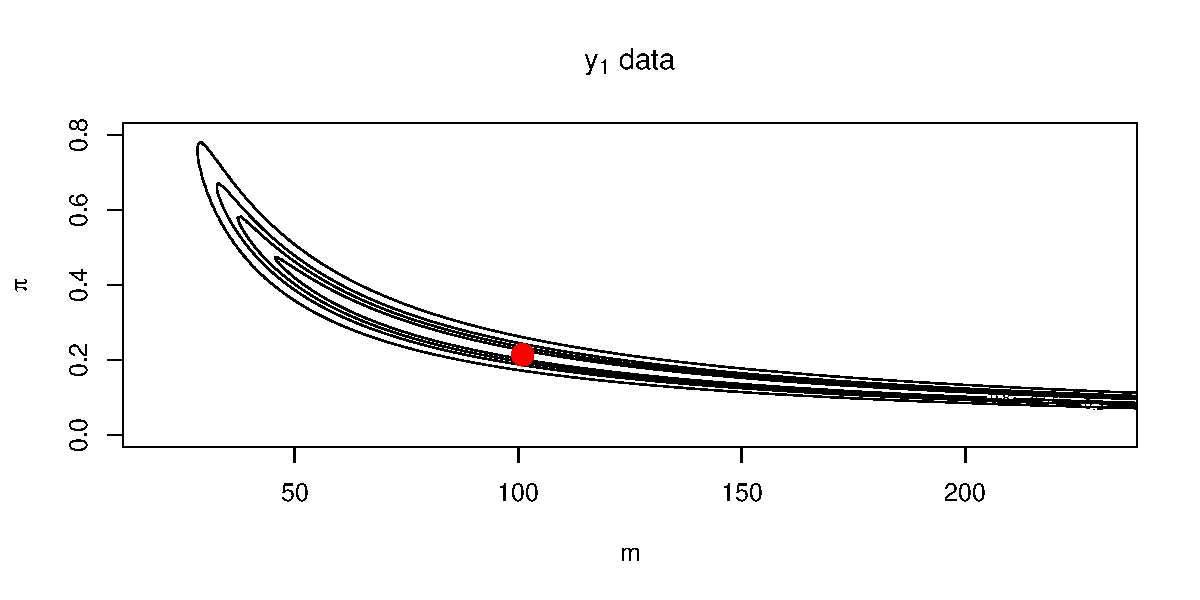
\includegraphics[width=.9\linewidth]{figure/likelihood-1} 

\end{knitrout}

\item The MLE occurs near $m=196, \pi=0.11$. I found this value by finding the maximum value on the grid.  

\begin{knitrout}\footnotesize
\definecolor{shadecolor}{rgb}{0.969, 0.969, 0.969}\color{fgcolor}
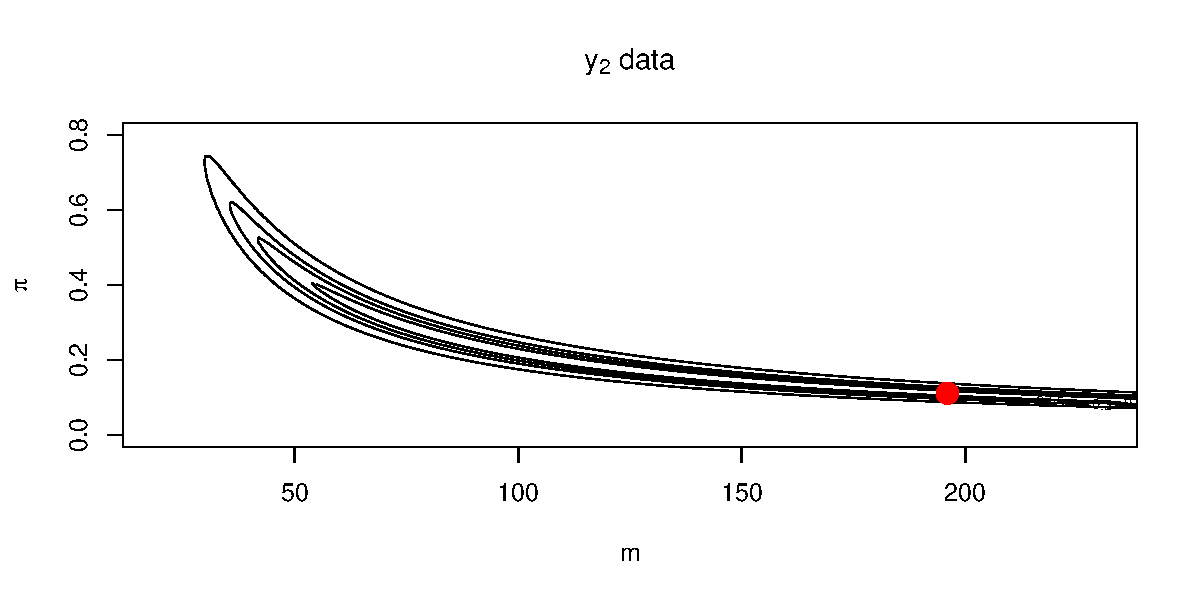
\includegraphics[width=.9\linewidth]{figure/likelihood2-1} 

\end{knitrout}

\item The shape of the likelihood function doesn't appear to change much in the contour plots, but my grid approximation for th MLE for $m$ changes from $101$ to $196$ when just one data point changes! Additionally, my grid approximation for the MLE for $\pi$ changes from $0.21$ to $0.11$.  I think this happens because the top of the likelihood function is fairly flat, so one small change in the data has a large effect on the location of the maximum. Because the top of the likelihood is so flat, I don't think it would be possible to use \verb+optim+ to solve for the MLE. I think the lesson here is that with so few data and $m$ and $\pi$ unknown, the MLE is very unstable and we shouldn't put too much trust in it.

\item \begin{enumerate}

\item The joint posterior distribution of $(m, \pi)$ is shown below, overlaid on the likelihood function from above. The posterior distribution is centered near the prior mean of $100$, and is actually far from the approximate MLE I found above. Additionally, the posterior contours are more circular and less spread out than the likelihood contour lines. Adding prior information seems to have improved the stability of the estimates for $m$ and $\pi$. 

\begin{knitrout}\footnotesize
\definecolor{shadecolor}{rgb}{0.969, 0.969, 0.969}\color{fgcolor}
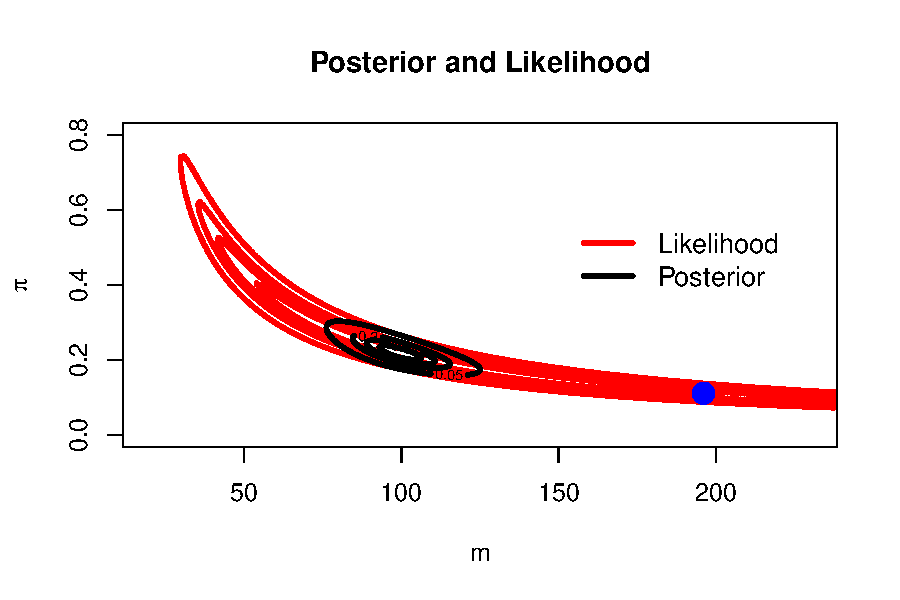
\includegraphics[width=.9\linewidth]{figure/jointpost-1} 

\end{knitrout}

\item My work for deriving the complete conditionals for $m$ and $\pi$ is shown below.
\begin{align*}
p(\pi|y, m) &= \frac{p(\pi, y, m)}{p(y, m)} \\
&\propto p(\pi, y, m) \\
&\propto p(y|\pi, m)p(m, \pi) \\
&\propto p(y|\pi, m)p(\pi) \\
&\propto \prod_{i=1}^{5} {m \choose y_i} \pi^{\sum  y_i} (1-\pi)^{\sum m-y_i} \\
p(m|y, \pi) &= \frac{p(\pi, y, m)}{p(y, \pi)} \\
&\propto p(\pi, y, m) \\
&\propto p(y|\pi, m)p(m, \pi) \\
&\propto p(y|\pi, m)p(m) \\
&\propto \prod_{i=1}^{5} {m \choose y_i} \pi^{\sum  y_i} (1-\pi)^{\sum m-y_i} \frac{e^{-100} 100^m}{m!}
\end{align*}

\item My code for the Gibbs sampler is shown below. I chose a Poisson proposal distribution for $m$ and a Beta proposal distribution for $\pi$.

\begin{knitrout}\footnotesize
\definecolor{shadecolor}{rgb}{0.969, 0.969, 0.969}\color{fgcolor}\begin{kframe}
\begin{alltt}
\hlcom{#function used previously to get log likelihood}
\hlstd{loglik.fun} \hlkwb{<-} \hlkwa{function}\hlstd{(}\hlkwc{m.pi}\hlstd{,} \hlkwc{y.vec}\hlstd{)\{}
  \hlkwd{sum}\hlstd{(}\hlkwd{lchoose}\hlstd{(m.pi[}\hlnum{1}\hlstd{], y.vec)}\hlopt{+}\hlstd{y.vec}\hlopt{*}\hlkwd{log}\hlstd{(m.pi[}\hlnum{2}\hlstd{])}\hlopt{+}\hlstd{(m.pi[}\hlnum{1}\hlstd{]}\hlopt{-}\hlstd{y.vec)}\hlopt{*}\hlkwd{log}\hlstd{(}\hlnum{1}\hlopt{-}\hlstd{m.pi[}\hlnum{2}\hlstd{]))}
\hlstd{\}}

\hlcom{#function used previously to get log prior}
\hlstd{log.prior.fun} \hlkwb{<-} \hlkwa{function}\hlstd{(}\hlkwc{m.pi}\hlstd{) \{}
  \hlopt{-}\hlkwd{lfactorial}\hlstd{(m.pi[}\hlnum{1}\hlstd{])}\hlopt{+}\hlstd{m.pi[}\hlnum{1}\hlstd{]}\hlopt{*}\hlkwd{log}\hlstd{(}\hlnum{100}\hlstd{)}\hlopt{-}\hlnum{100}
\hlstd{\}}

\hlcom{#function used previously to get log posterior}
\hlstd{log.post.fun} \hlkwb{<-} \hlkwa{function}\hlstd{(}\hlkwc{m.pi}\hlstd{,} \hlkwc{y.vec}\hlstd{) \{}
  \hlkwd{loglik.fun}\hlstd{(m.pi, y.vec)} \hlopt{+} \hlkwd{log.prior.fun}\hlstd{(m.pi)}
\hlstd{\}}

\hlcom{#function to calculate complete conditional for pi on log scale}
\hlstd{log.pi.cc.fun} \hlkwb{<-} \hlkwa{function}\hlstd{(}\hlkwc{m.pi}\hlstd{,} \hlkwc{y.vec}\hlstd{)\{}
  \hlkwd{loglik.fun}\hlstd{(m.pi, y.vec)}
\hlstd{\}}

\hlcom{#check function}
\hlcom{#log.pi.cc.fun(c(40, 0.5), y2.data)}

\hlcom{#function to calculate complete conditional for m on log scale}
\hlstd{log.m.cc.fun} \hlkwb{<-} \hlkwa{function}\hlstd{(}\hlkwc{m.pi}\hlstd{,} \hlkwc{y.vec}\hlstd{)\{}
  \hlkwd{log.post.fun}\hlstd{(m.pi, y.vec)}
\hlstd{\}}

\hlcom{#check function}
\hlcom{#log.m.cc.fun(c(40, 0.5), y2.data)}

\hlstd{nchain} \hlkwb{<-} \hlnum{3}
\hlstd{nsim} \hlkwb{<-} \hlnum{10000}
\hlstd{m.pi.mat} \hlkwb{<-} \hlkwd{array}\hlstd{(}\hlnum{NA}\hlstd{,} \hlkwc{dim}\hlstd{=}\hlkwd{c}\hlstd{(nsim,} \hlnum{2}\hlstd{, nchain))}

\hlcom{#keep track of acceptance ratios}
\hlstd{jump.mat} \hlkwb{<-} \hlkwd{matrix}\hlstd{(}\hlnum{NA}\hlstd{,} \hlkwc{nrow}\hlstd{=nsim}\hlopt{-}\hlnum{1}\hlstd{,} \hlkwc{ncol}\hlstd{=}\hlnum{2}\hlstd{)}

\hlcom{#specify starting values for each chain}
\hlstd{m.pi.mat[}\hlnum{1}\hlstd{,} \hlnum{1}\hlopt{:}\hlnum{2}\hlstd{,} \hlnum{1}\hlstd{]} \hlkwb{<-} \hlkwd{c}\hlstd{(}\hlnum{100}\hlstd{,} \hlnum{0.4}\hlstd{)}
\hlstd{m.pi.mat[}\hlnum{1}\hlstd{,} \hlnum{1}\hlopt{:}\hlnum{2}\hlstd{,} \hlnum{2}\hlstd{]} \hlkwb{<-} \hlkwd{c}\hlstd{(}\hlnum{50}\hlstd{,} \hlnum{0.2}\hlstd{)}
\hlstd{m.pi.mat[}\hlnum{1}\hlstd{,} \hlnum{1}\hlopt{:}\hlnum{2}\hlstd{,} \hlnum{3}\hlstd{]} \hlkwb{<-} \hlkwd{c}\hlstd{(}\hlnum{150}\hlstd{,} \hlnum{0.4}\hlstd{)}

\hlcom{#define standard deviations for normal proposal distributions}
\hlstd{sd.scale} \hlkwb{<-} \hlkwd{c}\hlstd{(}\hlnum{10}\hlstd{,} \hlnum{5}\hlstd{)}

\hlkwd{set.seed}\hlstd{(}\hlnum{230923}\hlstd{)}

\hlkwa{for} \hlstd{(j} \hlkwa{in} \hlnum{1}\hlopt{:}\hlstd{nchain) \{}
  \hlkwa{for} \hlstd{(i} \hlkwa{in} \hlnum{2}\hlopt{:}\hlstd{nsim) \{}
    \hlcom{#set pi equal to the starting value}
    \hlstd{pi} \hlkwb{<-} \hlstd{m.pi.mat[i}\hlopt{-}\hlnum{1}\hlstd{,} \hlnum{2}\hlstd{, j]}

    \hlcom{#now draw m from complete conditional with Metropolis Hastings Algorithm}
    \hlstd{m.cur} \hlkwb{<-} \hlstd{m.pi.mat[i}\hlopt{-}\hlnum{1}\hlstd{,} \hlnum{1}\hlstd{, j]}
    \hlstd{m.cand} \hlkwb{<-} \hlkwd{rpois}\hlstd{(}\hlnum{1}\hlstd{,} \hlkwc{lambda}\hlstd{=m.cur)}

    \hlstd{log.r.num.m} \hlkwb{<-} \hlkwd{log.m.cc.fun}\hlstd{(}\hlkwd{c}\hlstd{(m.cand, pi),} \hlkwc{y.vec} \hlstd{= y2.data)} \hlopt{+}
                     \hlkwd{dpois}\hlstd{(m.cur,} \hlkwc{lambda}\hlstd{=m.cand,} \hlkwc{log} \hlstd{=} \hlnum{TRUE}\hlstd{)}

    \hlstd{log.r.denom.m} \hlkwb{<-} \hlkwd{log.m.cc.fun}\hlstd{(}\hlkwd{c}\hlstd{(m.cur, pi),} \hlkwc{y.vec} \hlstd{= y2.data)} \hlopt{+}
                       \hlkwd{dpois}\hlstd{(m.cand,} \hlkwc{lambda}\hlstd{=m.cur,} \hlkwc{log} \hlstd{=} \hlnum{TRUE}\hlstd{)}

    \hlstd{log.r.m} \hlkwb{<-} \hlstd{log.r.num.m} \hlopt{-} \hlstd{log.r.denom.m}

    \hlstd{p.accept.m} \hlkwb{<-} \hlkwd{min}\hlstd{(}\hlnum{1}\hlstd{,} \hlkwd{exp}\hlstd{(log.r.m))}

    \hlstd{u.vec} \hlkwb{<-} \hlkwd{runif}\hlstd{(}\hlnum{2}\hlstd{)}

    \hlkwd{ifelse}\hlstd{(u.vec[}\hlnum{1}\hlstd{]} \hlopt{<=} \hlstd{p.accept.m, m.pi.mat[i,} \hlnum{1}\hlstd{, j]} \hlkwb{<-} \hlstd{m.cand,}
           \hlstd{m.pi.mat[i,} \hlnum{1}\hlstd{, j]} \hlkwb{<-} \hlstd{m.cur)}

    \hlstd{jump.mat[i}\hlopt{-}\hlnum{1}\hlstd{,} \hlnum{1}\hlstd{]} \hlkwb{<-} \hlkwd{ifelse}\hlstd{(u.vec[}\hlnum{1}\hlstd{]} \hlopt{<=} \hlstd{p.accept.m,} \hlnum{1}\hlstd{,} \hlnum{0}\hlstd{)}

    \hlcom{#now fix m at its value in the ith iteration}
    \hlstd{m} \hlkwb{<-} \hlstd{m.pi.mat[i,} \hlnum{1}\hlstd{, j]}

    \hlcom{#draw pi from complete conditional with metropolis hastings algorithm}
    \hlstd{pi.cur} \hlkwb{<-} \hlstd{m.pi.mat[i}\hlopt{-}\hlnum{1}\hlstd{,} \hlnum{2}\hlstd{, j]}
    \hlstd{pi.cand} \hlkwb{<-} \hlkwd{rbeta}\hlstd{(}\hlnum{1}\hlstd{,} \hlnum{2}\hlstd{, sd.scale[}\hlnum{2}\hlstd{])}

    \hlstd{log.r.num.pi} \hlkwb{<-} \hlkwd{log.pi.cc.fun}\hlstd{(}\hlkwd{c}\hlstd{(m, pi.cand),} \hlkwc{y.vec} \hlstd{= y2.data)} \hlopt{+}
                     \hlkwd{dbeta}\hlstd{(pi.cur,} \hlnum{2}\hlstd{, sd.scale[}\hlnum{2}\hlstd{],} \hlkwc{log} \hlstd{=} \hlnum{TRUE}\hlstd{)}

    \hlstd{log.r.denom.pi} \hlkwb{<-} \hlkwd{log.pi.cc.fun}\hlstd{(}\hlkwd{c}\hlstd{(m, pi.cur),} \hlkwc{y.vec} \hlstd{= y2.data)} \hlopt{+}
                       \hlkwd{dbeta}\hlstd{(pi.cand,} \hlnum{2}\hlstd{, sd.scale[}\hlnum{2}\hlstd{],} \hlkwc{log} \hlstd{=} \hlnum{TRUE}\hlstd{)}

    \hlstd{log.r.pi} \hlkwb{<-} \hlstd{log.r.num.pi} \hlopt{-} \hlstd{log.r.denom.pi}

    \hlstd{p.accept.pi} \hlkwb{<-} \hlkwd{min}\hlstd{(}\hlnum{1}\hlstd{,} \hlkwd{exp}\hlstd{(log.r.pi))}

    \hlstd{u.vec} \hlkwb{<-} \hlkwd{runif}\hlstd{(}\hlnum{2}\hlstd{)}

    \hlkwd{ifelse}\hlstd{(u.vec[}\hlnum{2}\hlstd{]} \hlopt{<=} \hlstd{p.accept.pi, m.pi.mat[i,} \hlnum{2}\hlstd{, j]} \hlkwb{<-} \hlstd{pi.cand,}
           \hlstd{m.pi.mat[i,} \hlnum{2}\hlstd{, j]} \hlkwb{<-} \hlstd{pi.cur)}

    \hlstd{jump.mat[i}\hlopt{-}\hlnum{1}\hlstd{,} \hlnum{2}\hlstd{]} \hlkwb{<-} \hlkwd{ifelse}\hlstd{(u.vec[}\hlnum{2}\hlstd{]} \hlopt{<=} \hlstd{p.accept.pi,} \hlnum{1}\hlstd{,} \hlnum{0}\hlstd{)}
  \hlstd{\}}
\hlstd{\}}
\end{alltt}
\end{kframe}
\end{knitrout}



\end{enumerate}

\item I checked convergence of my gibbs sampler and everything looks good. The marginal posterior distributions for $m$ and $\pi$ are shown below. The posterior mean for $m$ is $99.2$ and the posterior mean for $\pi$ is $0.22$. Recall that the approximate MLE I found on the grid was $m=196$, $\pi = 0.11$, and the prior means were $m = 100$ and $\pi = 0.5$. I display these means on the plot below. You can clearly see that the prior mean of $m$ has a huge influence on the posterior mean for $m$ (likely due to the instability in the likelihood based estimate for $m$). The prior mean for $\pi$ also has an impact on the posterior mean for $\pi$ (although a lesser impact than for $m$). \\

The posterior probability that $m>100$ is $0.443$ and the posterior probability that $\pi < 0.3$ is $0.989$. Since $m$ and $\pi$ are independent, the joint posterior probability that $m > 100$ and $\pi < 0.3$ is $0.443*0.989 = 0.438$.

\begin{knitrout}\footnotesize
\definecolor{shadecolor}{rgb}{0.969, 0.969, 0.969}\color{fgcolor}
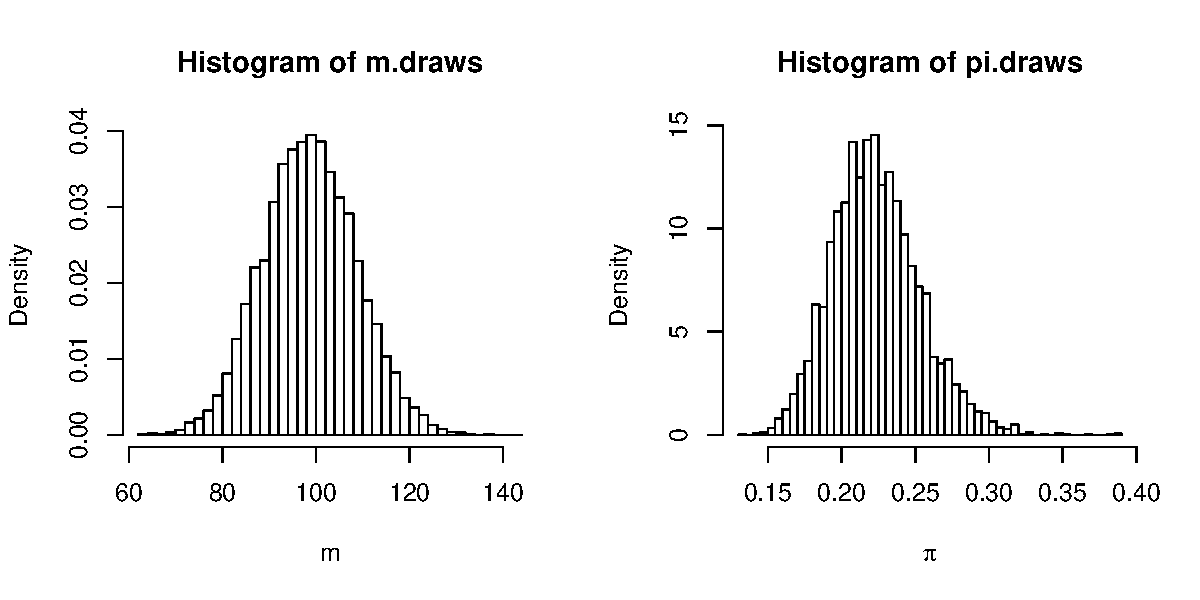
\includegraphics[width=\linewidth]{figure/converdiags-1} 

\end{knitrout}

\begin{knitrout}\footnotesize
\definecolor{shadecolor}{rgb}{0.969, 0.969, 0.969}\color{fgcolor}
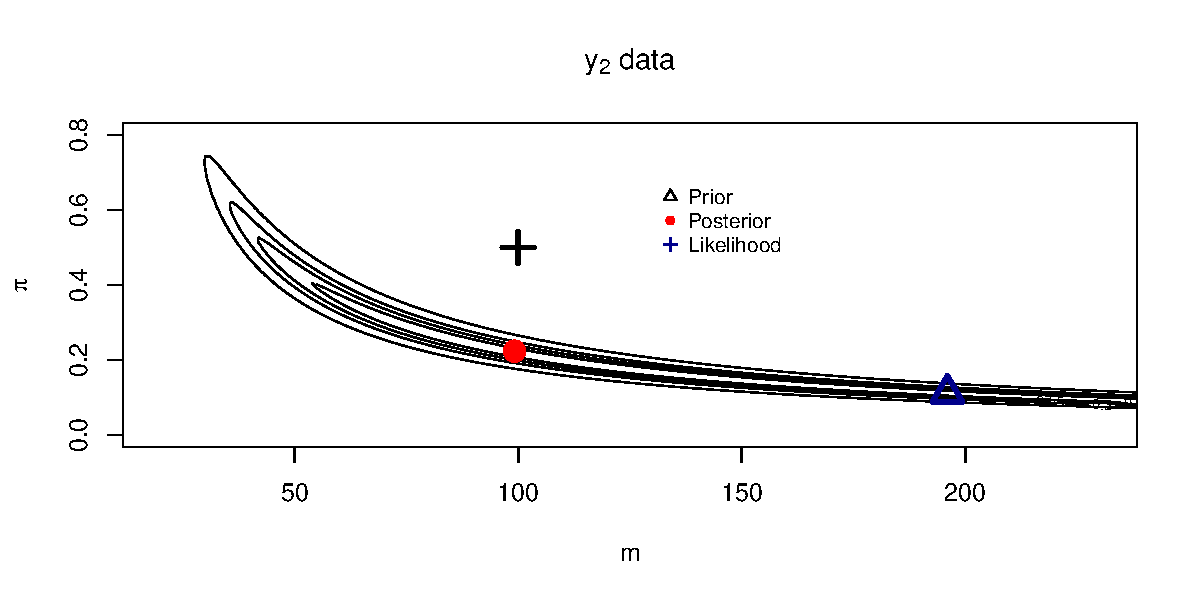
\includegraphics[width=\linewidth]{figure/contcompare-1} 

\end{knitrout}


\item The main disadvantage is that this model does not account for the fact that the values of the hyperparameters for $\pi$ and $m$ are unknown. $\lambda = 100$ was an estimated value, and the parameters of the Beta distribution were estimated as well. By treating these values as known, we are missing some uncertainty that should be incorporated in the model. I think another disadvantage of using the Poisson distribution as a prior is that the variance is a function of the mean, so that the variance of the prior can't be specified separately from the mean.

\item The hierarchical version of the model puts priors on $\lambda$ and priors on parameters of a $Beta(\alpha, \beta)$ distribution. I chose to put priors on the prior mean, $\eta = \frac{\alpha}{\alpha+\beta}$ and the somewhat approximate prior standard deviation, $\sigma = \sqrt{\frac{1}{\alpha + \beta}}$, kind of like what we did in the Beta-Binomial example with the stomach cancer data.
\begin{align*}
y_i &\sim Bin(m, \pi) \\
\pi &\sim Beta(\frac{\eta}{\sigma^2}, \frac{1-\eta}{\sigma^2}) \\
\sigma &\sim Uniform(0, 1) \\
\eta &\sim Uniform(0, 1) \\
m &\sim Poisson(\lambda) \\
\lambda &\sim Uniform(0, 500)
\end{align*}

I chose a $Uniform(0, 500)$ prior for $\lambda$ as a weakly informative prior. The Montana reservations aren't that large, and the number of eligible kids on each reservation can't be more than $500$. \\

I chose a $Uniform(0, 1)$ prior for the prior mean, $\eta$, to reflect little prior knowledge except that it must be between $0$ and $1$. I also put a $Uniform(0, 1)$ prior on the prior standard deviation, $\sigma$, to reflect little knowledge. At first, I experimented with putting a more diffuse prior on $\sigma$, but I had problems with convergence and the results weren't making sense. With values of $\pi$ between $0$ and $1$, I don't think it would make sense for the prior standard deviation to be larger than $1$. 

\item The JAGs code I used to obtain draws from the above model is shown below.

\begin{knitrout}\footnotesize
\definecolor{shadecolor}{rgb}{0.969, 0.969, 0.969}\color{fgcolor}\begin{kframe}
\begin{alltt}
\hlcom{##write model file first}
\hlkwd{cat}\hlstd{(}\hlstr{"
model
\{
for(i in 1:N)
\{
y[i] ~ dbin(pi, m)
\}

pi ~ dbeta(eta/sigma^2, (1-eta)/sigma^2)
eta ~ dunif(0, 1)
sigma ~ dunif(0, 1)

m ~ dpois(lambda)
lambda ~ dunif(0, 500)
\}"}\hlstd{,}
\hlkwc{file}\hlstd{=}\hlstr{"model1.jags"}\hlstd{)}
\end{alltt}
\end{kframe}
\end{knitrout}


\begin{knitrout}\footnotesize
\definecolor{shadecolor}{rgb}{0.969, 0.969, 0.969}\color{fgcolor}\begin{kframe}
\begin{alltt}
\hlcom{##jags call}
\hlkwd{library}\hlstd{(R2jags)}
\hlkwd{set.seed}\hlstd{(}\hlnum{52}\hlstd{)}


\hlstd{dental.data} \hlkwb{<-} \hlkwd{list}\hlstd{(}\hlkwc{N}\hlstd{=}\hlkwd{length}\hlstd{(y2.data),} \hlkwc{y}\hlstd{=y2.data)}

\hlstd{inits} \hlkwb{<-} \hlkwd{list}\hlstd{(}\hlkwd{list}\hlstd{(}\hlkwc{pi}\hlstd{=}\hlnum{0.4}\hlstd{,} \hlkwc{eta} \hlstd{=} \hlnum{.00003}\hlstd{,} \hlkwc{m} \hlstd{=} \hlnum{100}\hlstd{,} \hlkwc{lambda} \hlstd{=} \hlnum{500}\hlstd{,}
                   \hlkwc{sigma} \hlstd{=} \hlnum{0.5}\hlstd{),}
              \hlkwd{list}\hlstd{(}\hlkwc{pi}\hlstd{=}\hlnum{0.2}\hlstd{,} \hlkwc{eta} \hlstd{=} \hlnum{.02}\hlstd{,} \hlkwc{m} \hlstd{=} \hlnum{50}\hlstd{,} \hlkwc{lambda} \hlstd{=} \hlnum{150}\hlstd{,}
                   \hlkwc{sigma} \hlstd{=} \hlnum{0.9}\hlstd{),}
              \hlkwd{list}\hlstd{(}\hlkwc{pi}\hlstd{=}\hlnum{0.4}\hlstd{,} \hlkwc{eta} \hlstd{=} \hlnum{.5}\hlstd{,} \hlkwc{m} \hlstd{=} \hlnum{150}\hlstd{,} \hlkwc{lambda} \hlstd{=} \hlnum{300}\hlstd{,}
                   \hlkwc{sigma} \hlstd{=} \hlnum{0.1}\hlstd{))}
\hlstd{n.chain} \hlkwb{<-} \hlnum{3}

\hlcom{#warmup}
\hlstd{warmup.model1} \hlkwb{<-} \hlkwd{jags.model}\hlstd{(}\hlstr{"model1.jags"}\hlstd{,} \hlkwc{data}\hlstd{=dental.data,} \hlkwc{n.chains}\hlstd{=n.chain,}
                            \hlkwc{inits}\hlstd{= inits,} \hlkwc{n.adapt}\hlstd{=}\hlnum{4000}\hlstd{,} \hlkwc{quiet}\hlstd{=}\hlnum{TRUE}\hlstd{)}

\hlcom{#parameters to save}
\hlstd{params} \hlkwb{<-} \hlkwd{c}\hlstd{(}\hlstr{"pi"}\hlstd{,} \hlstr{"eta"}\hlstd{,} \hlstr{"sigma"}\hlstd{,} \hlstr{"m"}\hlstd{,} \hlstr{"lambda"}\hlstd{)}

\hlstd{n.iter}\hlkwb{=}\hlnum{50000}
\hlcom{#running the model for real}
\hlstd{model1} \hlkwb{<-} \hlkwd{coda.samples}\hlstd{(warmup.model1, params,} \hlkwc{n.iter}\hlstd{=n.iter)}
\end{alltt}
\end{kframe}
\end{knitrout}

\item The plots below compare the posterior distributions for $\pi$ and $m$ obtained in part (f) to those from the hierarchical model. There is much more variability in the posterior draws for $m$ and $\pi$ in the hierarchical model compared to the model with fixed hyperparameters. I think this makes sense because when the hyperparameter values are approximated, the model does not incorporate uncertainty in these parameters. With such a small sample size, the additional source of uncertainty accounted for in the hierarchical model makes a big difference in the results. \\

By allowing prior values of $\lambda$ to vary between $0$ and $500$, we see a large range of posterior draws for $m$ between $0$ and $500$. We do see a higher proportion of draws between $50$ and $100$. This is counterintuitive to me because with more uncertainty in the prior parameters, I would have expected the posterior for $m$ to be closer to the approximate MLE of $196$ that I found in part (c). For $\pi$, we do see a larger proportion of draws between $0.05$ and $0.2$, which is more similar to the MLE I estimated in part (c). 

\begin{knitrout}\footnotesize
\definecolor{shadecolor}{rgb}{0.969, 0.969, 0.969}\color{fgcolor}
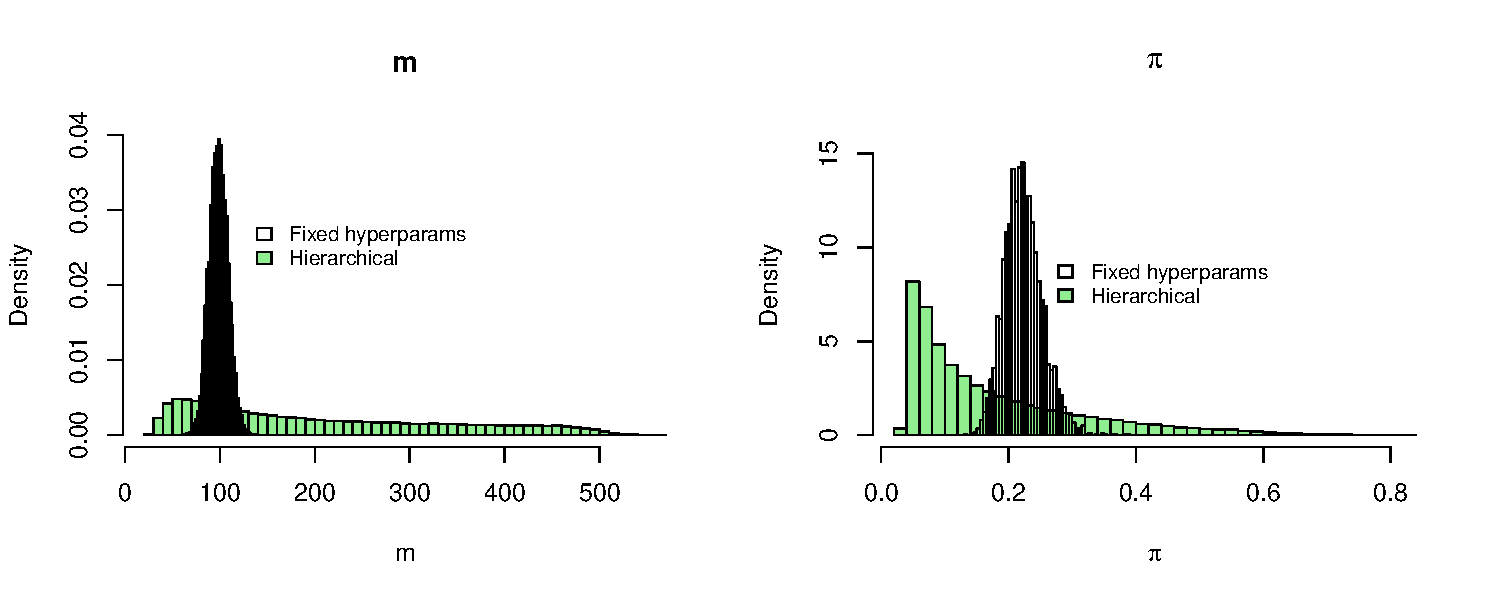
\includegraphics[width=\linewidth]{figure/jagsdrawscompare-1} 

\end{knitrout}

The posterior distributions of the hyperparameters are shown below, with the fixed values used in (e). The fixed values used in (e) are well within the range of posterior draws for the hyperparameters. Looking at these plots, it's really apparent how much additional uncertainty is incorporated into the model by putting hyperpriors on the hyperparameters instead of treating them as known. 

\begin{knitrout}\footnotesize
\definecolor{shadecolor}{rgb}{0.969, 0.969, 0.969}\color{fgcolor}
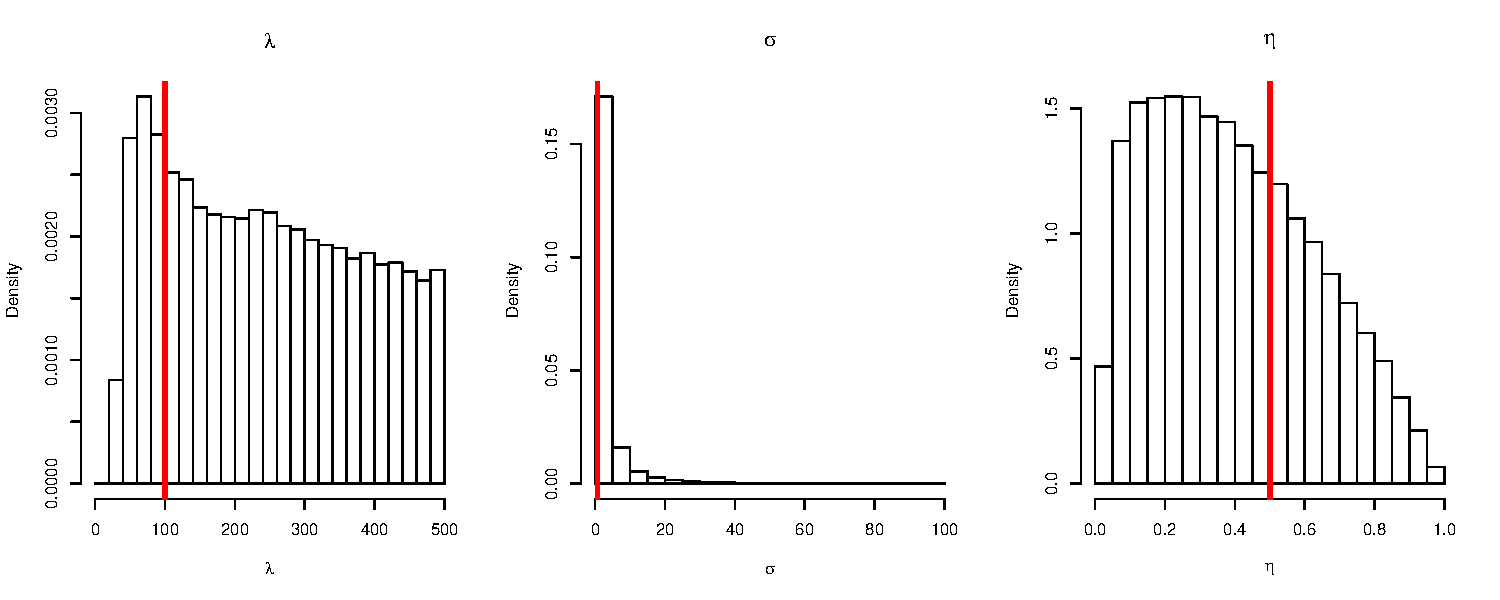
\includegraphics[width=\linewidth]{figure/jagshyperdraws-1} 

\end{knitrout}

\item \begin{enumerate}

\item When I first looked at this prior, I thought he was trying to give higher density to values of $\lambda$ and $\pi$ that yield smaller expected numbers of successes. But then, on second thought, I thought maybe this prior is similar to the $\frac{1}{\sigma^2}$ prior which does give higher density to small values of $\sigma^2$, but is actually a non-informative prior because it spreads density throughout a large range of parameter values. I think a good way to visualize this would be to write rejection sampling code to sample from this prior, and see what combinations of $\pi$ and $\lambda$ are sampled most often. We could also look at the sensitivity of the posterior to the prior to get a sense of whether it is acting as a ``non-informative'' prior. \\

\item When I look at the plot of the Raftery Prior, it looks like small values of $\lambda$ with any value of $\pi$ are most probable because the contour lines show up in the farthest left portion of the plot. When I generated draws from the priors I specified in (i), I get a smattering of values of $\lambda$ and $\pi$ over the entire parameter space. My prior appears to be more vague than the raftery prior, with probability spread more evenly throughout the parameter space.


\begin{knitrout}\footnotesize
\definecolor{shadecolor}{rgb}{0.969, 0.969, 0.969}\color{fgcolor}
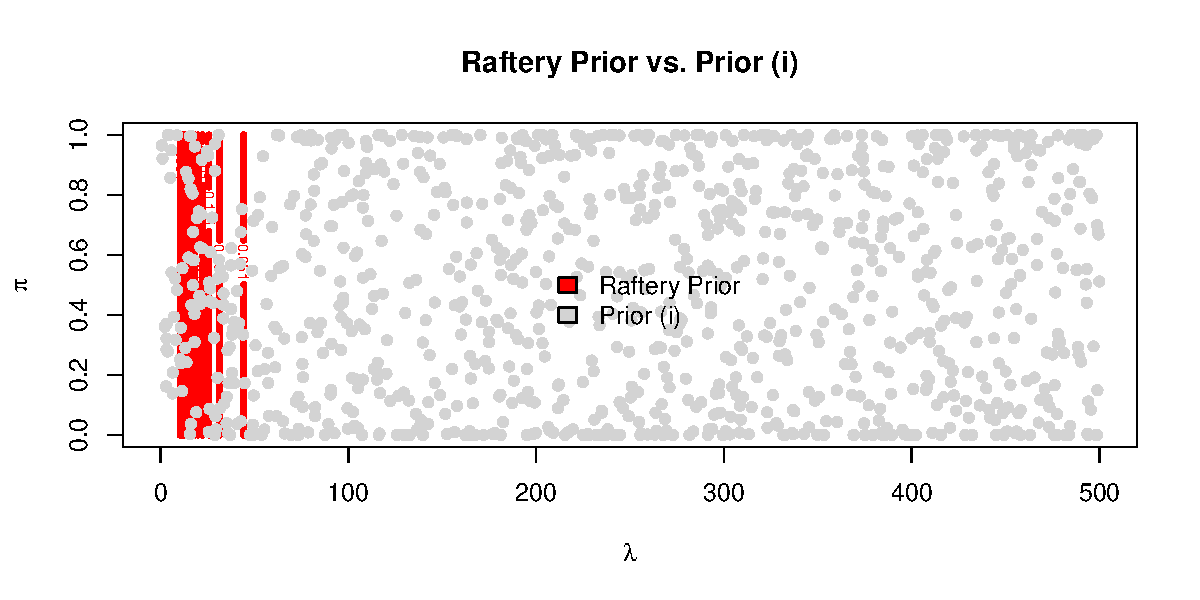
\includegraphics[width=0.8\linewidth]{figure/drawfrommultiprior-1} 

\end{knitrout}


\end{enumerate}

\end{enumerate}

\item \begin{enumerate}

\item The simple logistic regression model for estimating the dose-death relationship is as follows. I treat dose as a continuous predictor variable. The empirical probabilities of death at each dose as well as the fitted probabilities from the glm() model are shown on the plot below. The dose at which half of the frogs are estimated to die is $\frac{0.5 + 56.97}{78.29} = 0.734$ grams per ml. 
\begin{align*}
y_{ij} \sim& Bin(5, \pi_j) \\
logit(\pi_j) &= \alpha + \beta x_j
\end{align*}



\begin{knitrout}\footnotesize
\definecolor{shadecolor}{rgb}{0.969, 0.969, 0.969}\color{fgcolor}\begin{kframe}


{\ttfamily\noindent\color{warningcolor}{\#\# Warning: glm.fit: fitted probabilities numerically 0 or 1 occurred}}\end{kframe}
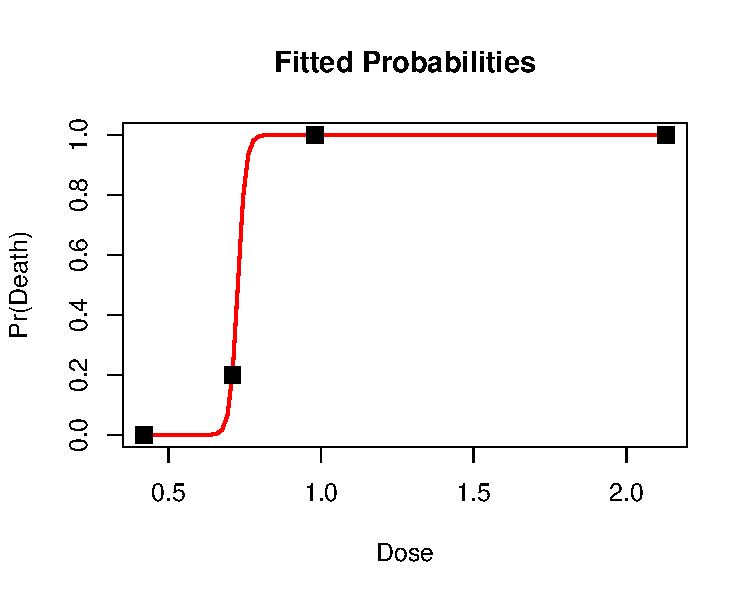
\includegraphics[width=.5\linewidth]{figure/glmmodel-1} 

\end{knitrout}

\item The model I will use to do the analysis in a Bayesian framework is shown below. 
\begin{align*}
y_{ij} &\sim Bern(logit^{-1}(\alpha + \beta x_j)) \\
p(\alpha) &\propto 1 \\
p(\beta) &\propto 1
\end{align*}

\item The model code is shown below.
\begin{knitrout}\footnotesize
\definecolor{shadecolor}{rgb}{0.969, 0.969, 0.969}\color{fgcolor}\begin{kframe}
\begin{alltt}
data \{
  int<lower=0> N;
  vector[N] x;
  int<lower=0,upper=1> y[N];
\}
parameters \{
  real alpha;
  real beta;
\}
model \{
  y ~ \hlkwd{bernoulli_logit}(alpha + beta * x);
\}
\end{alltt}
\end{kframe}
\end{knitrout}


\begin{knitrout}\footnotesize
\definecolor{shadecolor}{rgb}{0.969, 0.969, 0.969}\color{fgcolor}\begin{kframe}
\begin{alltt}
\hlkwd{require}\hlstd{(rstan)}
\hlkwd{set.seed}\hlstd{(}\hlnum{23}\hlstd{)}
\hlstd{data} \hlkwb{<-} \hlkwd{with}\hlstd{(frog.data,} \hlkwd{list}\hlstd{(}\hlkwc{y} \hlstd{= death,} \hlkwc{x} \hlstd{= dose,} \hlkwc{N} \hlstd{=} \hlkwd{length}\hlstd{(death)))}

\hlstd{model2} \hlkwb{<-} \hlkwd{stan_model}\hlstd{(}\hlkwc{file} \hlstd{=} \hlstr{"~/Documents/Stat532/exams/exam2/model2.stan"}\hlstd{,}
                     \hlkwc{model_name} \hlstd{=} \hlstr{"model2"}\hlstd{)}
\hlstd{samp2} \hlkwb{<-} \hlkwd{sampling}\hlstd{(model2,} \hlkwc{chains} \hlstd{=} \hlnum{4}\hlstd{,} \hlkwc{iter} \hlstd{=} \hlnum{2000}\hlstd{,} \hlkwc{data} \hlstd{= data)}
\end{alltt}
\end{kframe}
\end{knitrout}

\item The posterior draws for the y-intercept ($\alpha$) and the dose effect ($\beta$) are shown below. The red line indicates the estimate from the above generalized linear model. Note that the posterior draws seem really extreme. When I ran the model, I got a warning message that said, ``There were 8332 transitions after warmup that exceeded the maximum treedepth". I looked at the traceplots, and they indicated that the model  had not converged. I think convergence is taking a long time because the priors used are so diffuse, and I think the warning message is happening because the data have separation issues.

\begin{knitrout}\footnotesize
\definecolor{shadecolor}{rgb}{0.969, 0.969, 0.969}\color{fgcolor}
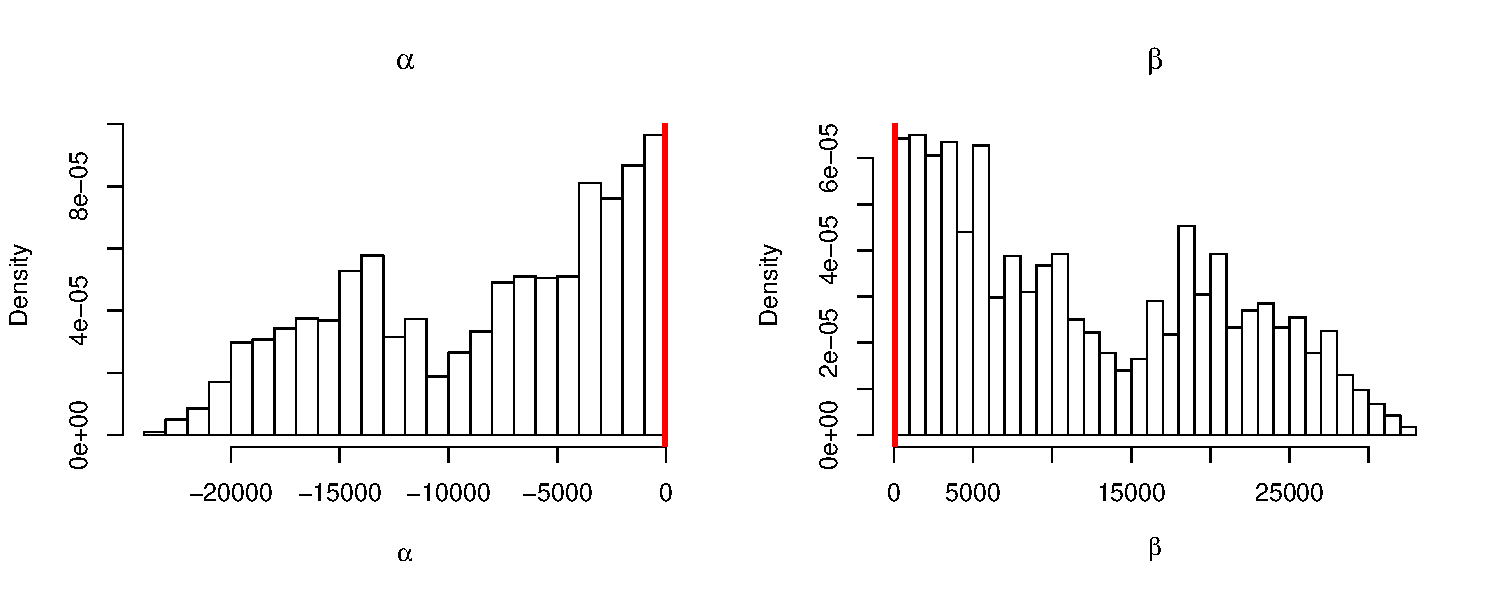
\includegraphics[width=\linewidth]{figure/compare-1} 

\end{knitrout}

\item Most of the posterior draws for $\alpha$ and $\beta$ were way more extreme than the estimates from the traditional logistic regression model. I think these extreme draws are occuring in the STAN model because the posterior distributions are sensitive to the prior when a small amount of data are available. With such diffuse priors on $\alpha$ and $\beta$, very extreme values are considered probable. In contrast, the binomial logistic regression model fits a line to the empirical logits, and no other information other than the data is supplied when estimating $\alpha$ and $\beta$. So, without the influence of a large diffuse prior, the observed values of $\alpha$ and $\beta$ are less extreme. \\

I started to compare the mean LD50 in the stan model to the estimated LD50 found from glm(). Recall the estimated LD50 from glm() was $0.734$. From the STAN model, I found that the estimated LD50 from all the posterior draws was $0.711$ with a $95\%$ posterior interval from $0.710$ to $0.717$! I thought this was really weird, so I looked at a two dimensional plot of the ($\alpha, \beta$) draw pairs (see below). It seems like what happened in this model is that the extreme draws were drawn in pairs, and were all proportional to the estimates found from glm(). In any case, strange things are happening with such diffuse priors, and I think we should consider more informative priors, especially when there are so few data.

\begin{knitrout}\footnotesize
\definecolor{shadecolor}{rgb}{0.969, 0.969, 0.969}\color{fgcolor}
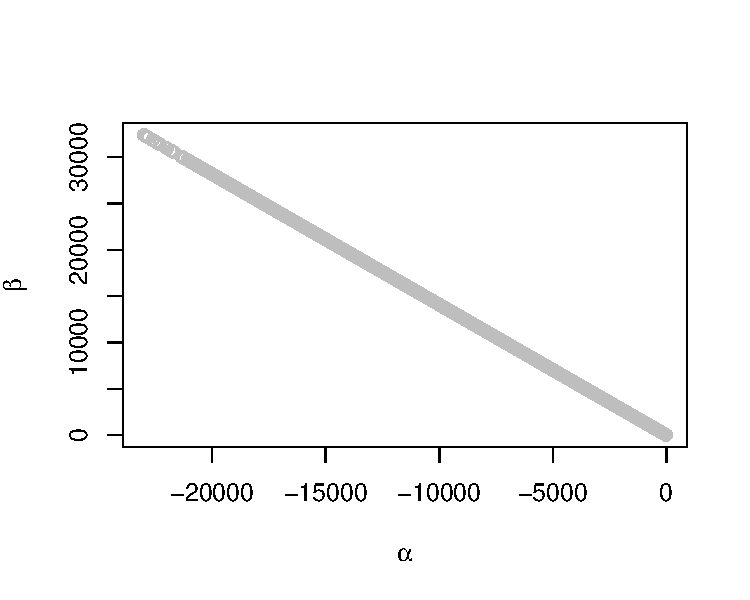
\includegraphics[width=.5\linewidth]{figure/mat-1} 

\end{knitrout}


\item The plots of the posterior draws for $\alpha$ and $\beta$ are shown below for the model with standardized dose as the predictor variable. The posterior draws for $\alpha$ have changed, but this is expected because $\alpha$ is now the log odds of death at the average dose. The posterior draws for $\beta$ have also changed, but this is also expected because now $\beta$ represents the increase in the log odds of survival for a one standardized unit increase in dose. \\

I used the LD50 to compare inference between the first model and the model with standardized dose. I found the LD50 on the standardized scale first, and then transformed back to dose on the original scale. After doing so, I found that the mean LD50 is estimated to be $0.7100$, with a $95\%$ posterior interval from $0.7100$ to $0.7102$. Because these results are very similar to what I saw before dose was standardized, I conclude that standardizing dose does not change inference in this case. Also, the efficiency of the sampler has not changed noticeably.



\begin{knitrout}\footnotesize
\definecolor{shadecolor}{rgb}{0.969, 0.969, 0.969}\color{fgcolor}
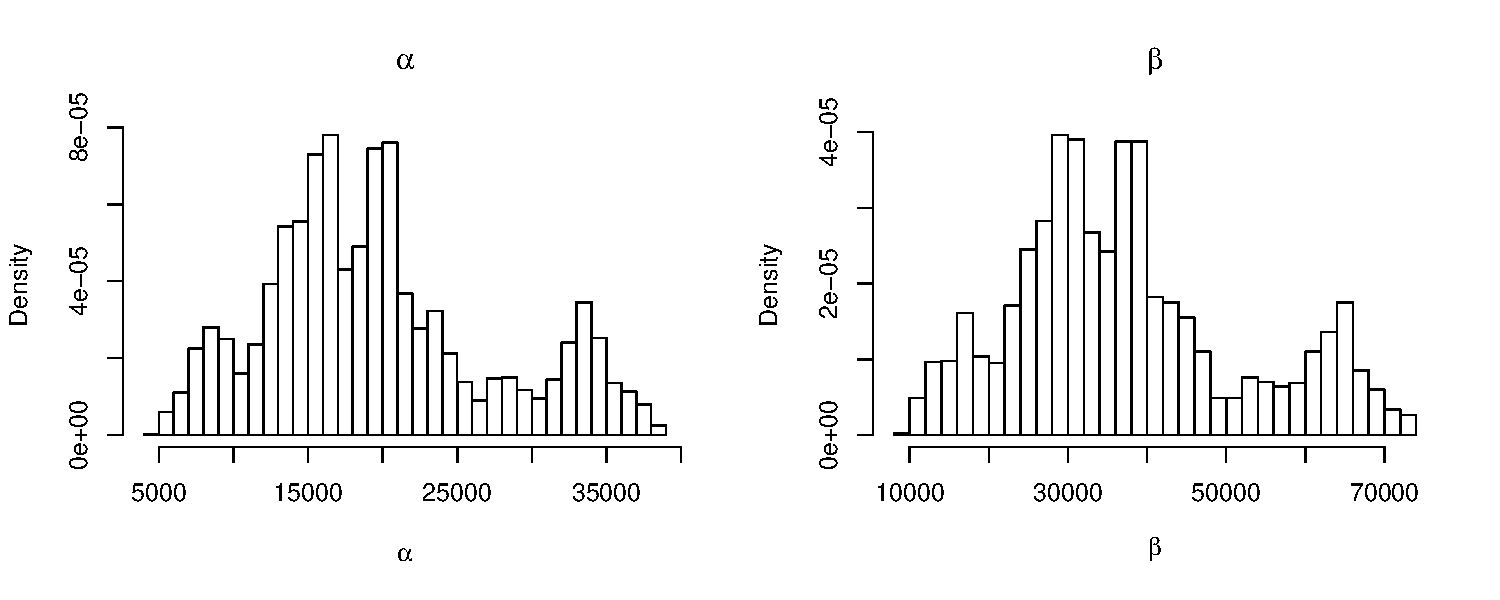
\includegraphics[width=\linewidth]{figure/stdcompare-1} 

\end{knitrout}

\item The cauchy priors are shown below. For the intercept, the $Cauchy(0, 10)$ prior allows for the possibility of any value over the whole real line, but the probable values for the intercept are between $-30$ and $30$. This is a huge spread on the logit scale, and if we transform back to the original scale, this prior allows for the probability of death at the average dose to be between $logit^{-1}(-30) = 9.4*10^{-14}$ and $logit^{-1}(30) \approx 1$! With such a large spread on the original scale, this prior is weakly informative because it incorporates the natural constraints that the probability of death must be between $0$ and $1$. \\

For the slope, the probable prior values are between $-20$ and $20$ on the logit scale. This means that for a one standardized unit increase of dose, the odds of death can change by a multiplicative factor between the values of $e^{-10} = 4.54*10^{-5}$ and $e^{10} = 22026.5$. With the prior density spread out over such a large range over values, very little prior is incorporated about the dose effect. It does incorporate the natural constraint that the change in the odds must be greater than $0$. For this parameter, I think we could do a better job at incorporating the prior knowledge that $\beta > 0$ (it's a lethal toxin). I come up with a better weakly informative prior in part (i).  

\begin{knitrout}\footnotesize
\definecolor{shadecolor}{rgb}{0.969, 0.969, 0.969}\color{fgcolor}
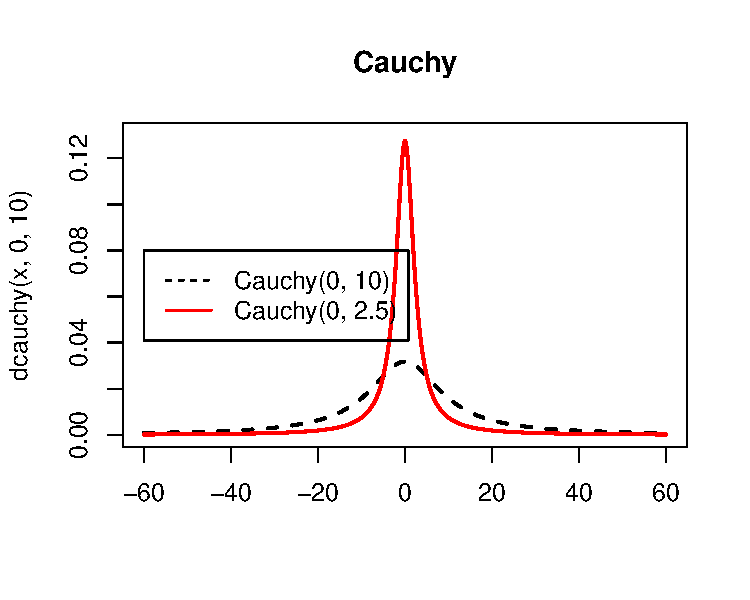
\includegraphics[width=.5\linewidth]{figure/dcauchy-1} 

\end{knitrout}

\item The posterior distributions of $\alpha$ and $\beta$ are shown below. The regression lines displaying the fitted logits, and the fitted probability curves for all $4000$ posterior draws are also shown. \\

These results look way more reasonable than the previous results found using the improper priors. I think it's amazing that the results can change so much when transitioning from an uninformative to a weakly informative prior. The posterior mean for $\alpha$ is $-10.81$, with a 95\% posterior interval from $-27.74$ to $-2.28$, and the posterior mean for $\beta$ is $13.90$ with a $95\%$ posterior interval from $2.94$ to $37.72$. The posterior mean LD50 is $0.84$ with a $95\%$ posterior interval from $0.70$ to $1.01$.\\
 
In this case, most of the posterior draws for $\alpha$ and $\beta$ are actually less extreme than the estimates from the glm() model. I think it's more reasonable that the fitted probability curves aren't as steep as the fitted curve from the glm() model (see plots below). The model seems to take into account that few data are available and the probability of death isn't {\it exactly} $1$ at a dose of $1$. In the glm() model, however, the fitted curve is so steep because it is forced to go through (or get close to) the point at (1, 1). In the Bayesian model, with the ability to incorporate prior knowledge, it's kind of like we can help the model to reflect the fact that the data don't always represent the true relationship. 



\begin{knitrout}\footnotesize
\definecolor{shadecolor}{rgb}{0.969, 0.969, 0.969}\color{fgcolor}
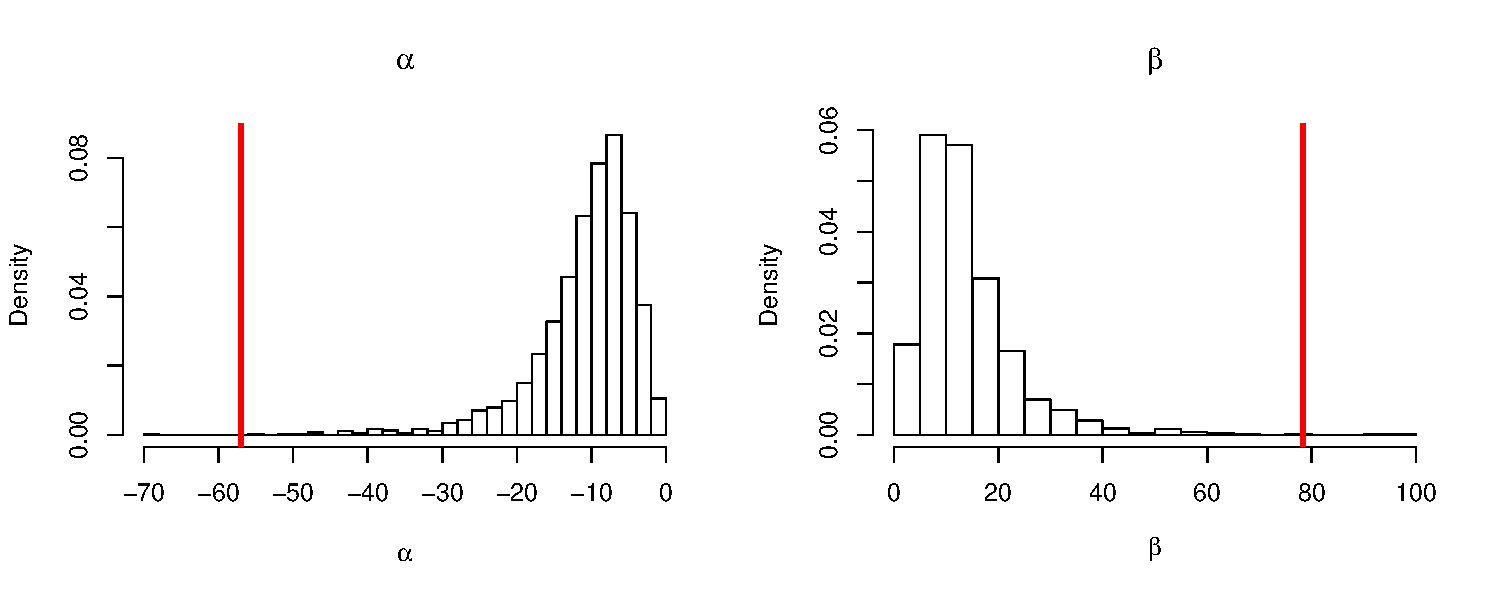
\includegraphics[width=\linewidth]{figure/compare4-1} 

\end{knitrout}

\begin{knitrout}\footnotesize
\definecolor{shadecolor}{rgb}{0.969, 0.969, 0.969}\color{fgcolor}
\includegraphics[width=\linewidth]{figure/plotreglines-1} 

\end{knitrout}

\item I'll use the Cauchy prior for $\alpha$ again with a smaller scale parameter. I'll use the Cauchy(0, 2) prior for $\alpha$, which makes the more likely values for $\alpha$ (the probability of death at a dose of $0$) to be between about $0.01$ and $0.99$. This is still not very informative, but it is more informative than the Cauchy(0, 10). For $\beta$, I'll use a folded Cauchy prior. The problem does state that this drug is known to be lethal to frogs, so we should incorporate into our prior the knowledge that $\beta$ is greater than $0$. I'll use a folded Cauchy(0, 2.5). I'm still reflecting little knowledge in the magnitude of $\beta$, but this prior is more informative in the sense that it does not allow for negative values of $\beta$. The results are shown below for this model. \\

Also, I'd like to note that I realize problem (g) told us to standardize dose, but I don't think it's necessary, and the results are easier to interpret and compare across models if I don't standardize.

\begin{knitrout}\footnotesize
\definecolor{shadecolor}{rgb}{0.969, 0.969, 0.969}\color{fgcolor}
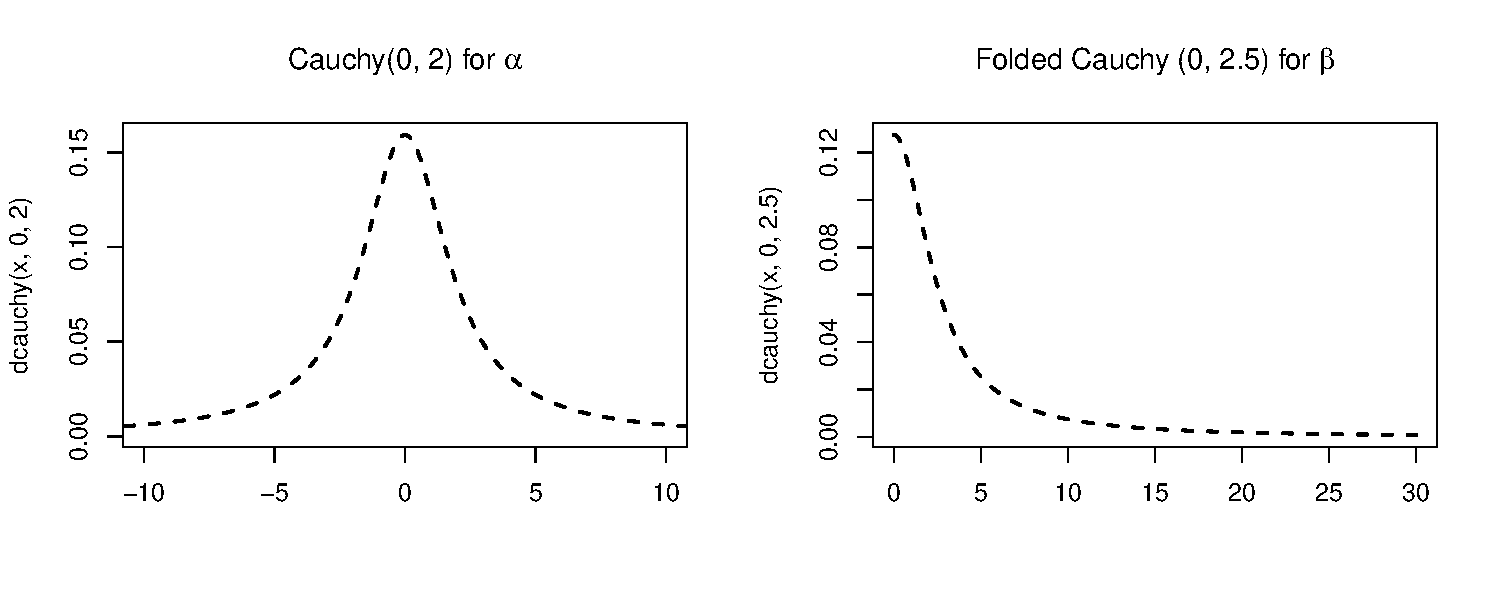
\includegraphics[width=\linewidth]{figure/cauchyagain-1} 

\end{knitrout}




The posterior mean for $\alpha$ is $-7.71$, which indicates that the probability of death at a dose of $0$ is estimated to be $0.00045$, with a $95\%$ posterior interval from $4*10^{-10}$ to $0.18$. The posterior mean for $\beta$ is $9.95$, which indicates that the odds of death are estimated to increase by a multiplicative factor of $2.7$ when dose increases by $0.1$ g/ml, with a $95\%$ posterior interval from $1.24$ to $16.62$ times. The dose at which $50\%$ of frogs are expected to die is estimated to be $0.85$ g/ml, with a $95\%$ posterior interval from $0.66$ to $1.14$ g/ml.


\begin{knitrout}\footnotesize
\definecolor{shadecolor}{rgb}{0.969, 0.969, 0.969}\color{fgcolor}
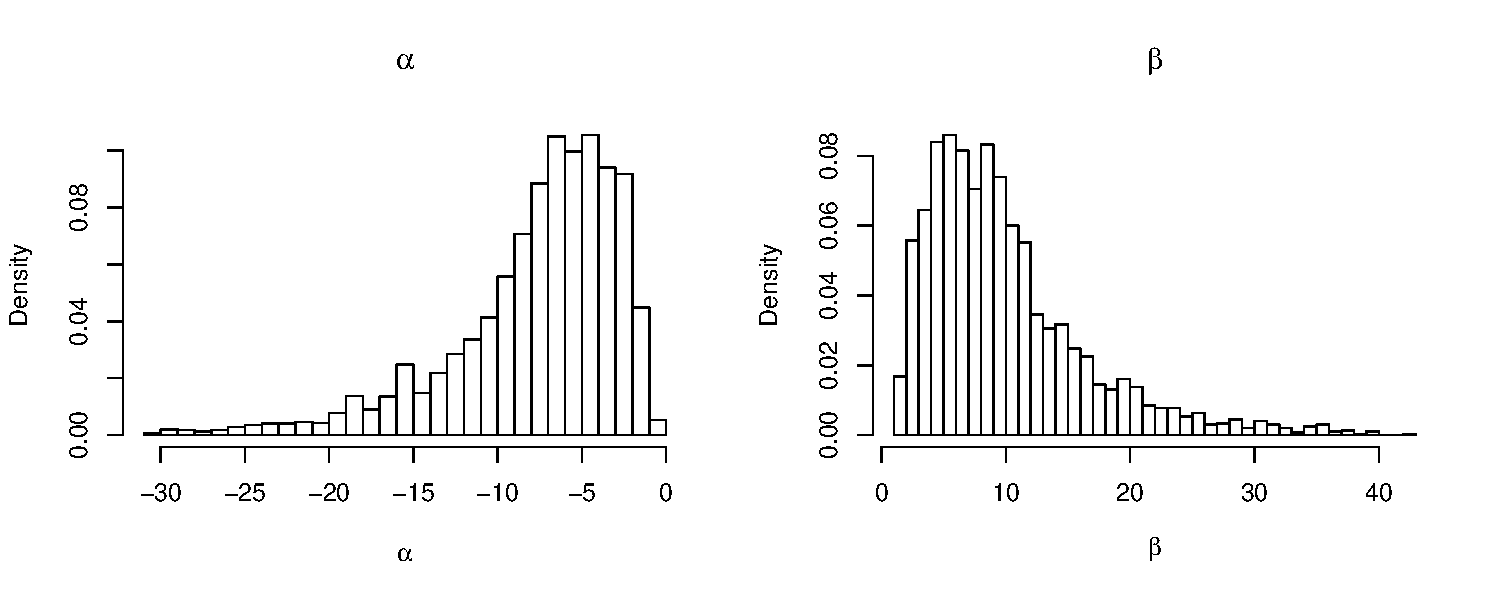
\includegraphics[width=\linewidth]{figure/compare5-1} 

\end{knitrout}



\begin{knitrout}\footnotesize
\definecolor{shadecolor}{rgb}{0.969, 0.969, 0.969}\color{fgcolor}
\includegraphics[width=\linewidth]{figure/plotreglinesinform-1} 

\end{knitrout}



\item In the histograms below, I compare the results for the models from (g) and (i). You can see the posterior draws of $\alpha$ and $\beta$ are drawn closer to $0$ in the model from part (i). \\

I think the analysis in part (i) is most appropriate. The results from the improprer priors in part (c) do not make sense, not to mention I get a warning message when I run the model. The results from the Cauchy priors in part (g) are reasonable, but I think the prior I chose in part (i) is more appropriate because I chose priors that incorporated reasonable constraints in the context of the problem but were still vague enough to reflect little prior knowledge. The Cauchy priors in part (g) were more diffuse than they needed to be to reflect little prior knowlege in this context. I guess this is just another situation where it's smarter to think carefully about your priors instead of just choosing default non-informative priors.

\begin{knitrout}\footnotesize
\definecolor{shadecolor}{rgb}{0.969, 0.969, 0.969}\color{fgcolor}
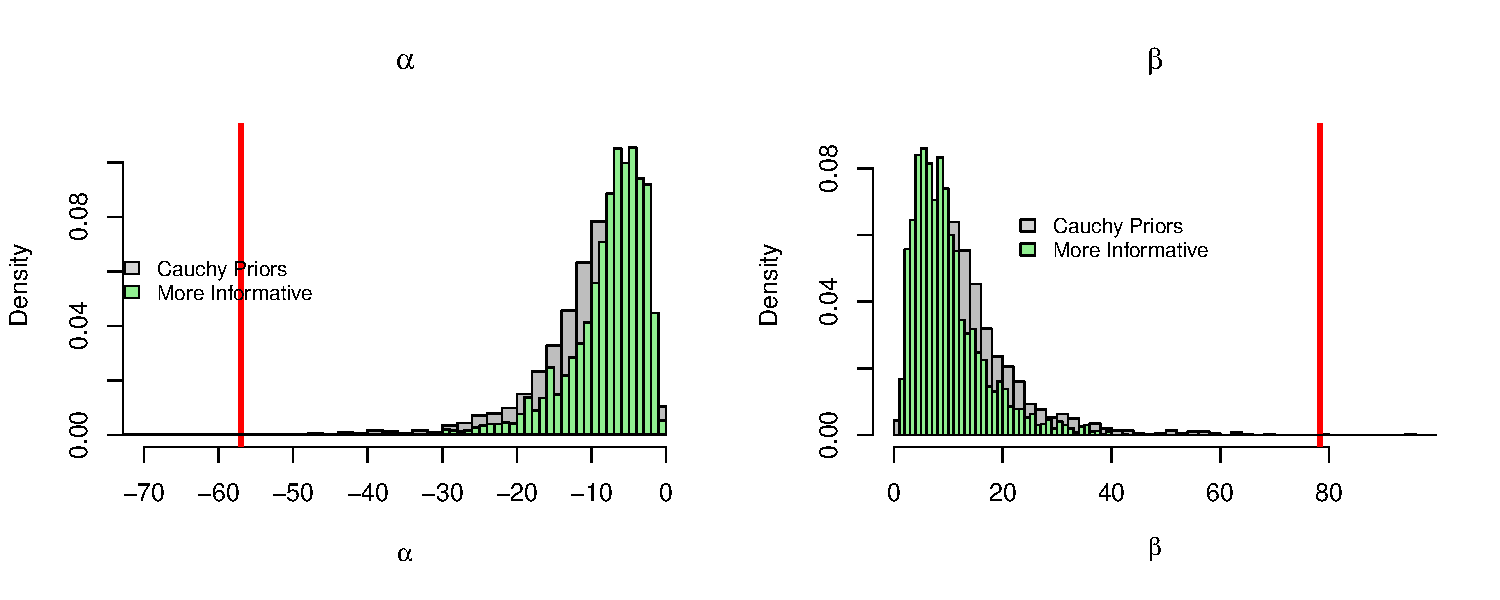
\includegraphics[width=\linewidth]{figure/compareall-1} 

\end{knitrout}


\item I do not expect the assumption of independence to be met because I would expect the frogs in the same tank to have more similar death rates than frogs in different tanks. There could be other sources of dependence in the design that we are not told about such as age or health of the frogs. For this problem, I'll focus on investigating whether the death rates are more similar for frogs in the same tank. \\

To implement the posterior predictive check, I will generate a large number of posterior predictive samples. For each posterior predictive sample, I'll assume that the first three frogs within a dose came from tank $1$, and the last two frogs within that dose came from tank $2$. Then, for each posterior predictive sample, I'll calculate the number of deaths within each tank for each dose. I'll display the histograms showing the distribution of deaths within each tank at each dose for all posterior predictive samples. I'll then compare to what was observed in the original dataset. My posterior predictive displays will look something like the following. I simulated these posterior predictions for the purpose of example, and I also show the code here.



\begin{knitrout}\footnotesize
\definecolor{shadecolor}{rgb}{0.969, 0.969, 0.969}\color{fgcolor}
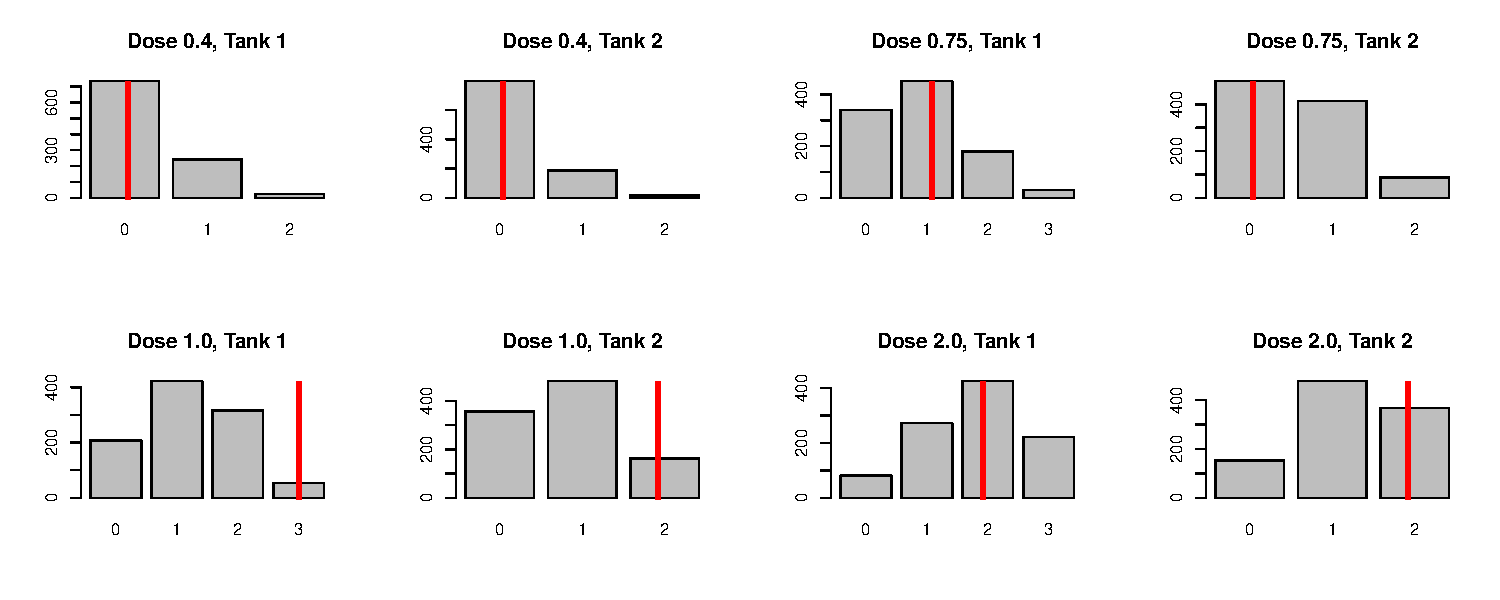
\includegraphics[width=\linewidth]{figure/exdisplay-1} 

\end{knitrout}

Since the model generates posterior predictions under the assumption of independent observations, the posterior predictions represent what we would expect to see if frog deaths occurred independently within tanks. If the observed data showed more tanks with all frogs dying or no frogs dying than predicted by the model, I would suspect dependence among frogs within a tank. For example, suppose the number of deaths were most often $1$ death per tank in the posterior predictive samples. Then, if we observed either all or none of the frogs dying within a tank in the original sample, I would suspect that one frog dying in the tank is affecting the probability of death for another frog in that tank. An example of this would be the barplot shown for Dose 1.0, Tank 1 in the above figure. Biologically, I think it seems reasonable that if one frog dies within a tank and is not cleaned out right away, it would decrease the overall health of the other frog(s) in the tank and increase their probability of death.

\item A fully Bayesian hierarchical model would be as follows. This model incorporates an adjustment for each tank ($k=1,2$), and it accounts for uncertainty in the parameters for the population of tank adjustments.
\begin{align*}
y_{ijk} &\sim Bern(logit^{-1}(\alpha + \beta x_j + \gamma_k)) \\
\alpha &\sim Cauchy(0, 2) \\
\beta &\sim Cauchy(0, 2.5) \\
\gamma_k &\sim N(0, \sigma^2) \\
p(\sigma) &\propto 1
\end{align*}

\end{enumerate}

\item \begin{enumerate}

\item Take for example the $N(0, 10000)$ prior that people sometimes use as a default 'uninformative prior' in canned software packages when they are forced to choose a proper prior. The relative density does appear to be higher for values of the parameter near $0$ (see below). But, the difference in densities is very small because the prior is spread out over such a large range of values (note the peak density is around $0.00004$). As a result, the chance of drawing a value between $0$ and $10$ isn't that much different than the chance of drawing a value between $20000$ and $20010$. This prior is uninformative in the sense that a very wide range of prior values are probable, and the difference in densities over this very wide range of values is small because the prior is so diffuse.  

\begin{knitrout}\footnotesize
\definecolor{shadecolor}{rgb}{0.969, 0.969, 0.969}\color{fgcolor}
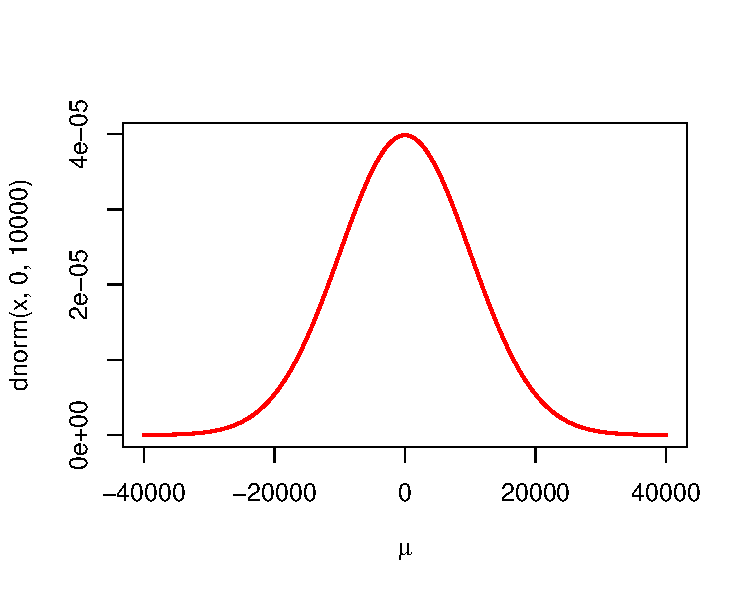
\includegraphics[width=.5\linewidth]{figure/stdprior-1} 

\end{knitrout}

\item The posterior is sometimes sensitive to priors that are commonly regarded as non-informative. Take for example the $InvGam(0.01, 0.01)$ prior that is commonly used as a non-informative prior for variance parameters. Recent work has shown that applying this prior to a group level variance parameter in a hiearchical model can lead to very different posterior distributions than if a different vague, diffuse prior is used (Gelman 2006). This goes to show that a sensitivity analysis of the posterior to the priors should be performed even if the priors used are commonly known as non-informative.

\end{enumerate}

\item The proposal distribution is a computational tool used to obtain draws from the posterior distribution. We need to get the spread and center of the proposal distribution just right to maximize efficiency of the Metropolis Hastings algorithm. So, we often look at the likelihood to get a ballpark idea of what the spread of the proposal distribution should be. The key difference between the proposal distribution and the prior distribution is that the proposal distribution does not contribute to the model at all, it is simply used in computation. If we try to use the likelihood to inform the prior distribution, you are essentially using the data to inform the model. This is called an empirical Bayes approach and is not a true Bayesian analysis.

\item The data won't always be representative of the population, and with few data it is hard to quantify the amount of variability in the population. As a result, classical inference is often wrong if few data available and are not representative of the population. The ability to incorporate prior knowledge in a Bayesian analysis can help us see when the data collected are not representative of the truth, and it can help us fit a better, more informed model. I think of the prior as a piece of known information going into the fitted model. As I saw in problems $1$ and $2$, the prior can really help to inform results and lead to reasonable posteriors even when the few data available don't seem to provide much information at all.

\end{enumerate}

\newpage

{\Large \bf References} \\

\noindent Gelman, Andrew. "Prior Distributions for Variance Parameters in Hierarchical Models(Comment on Article by Browne and Draper)." International Society for Bayesian Analysis 1.3 (2006): 515-34. Print.

{\Large \bf R Code Appendix}

\begin{knitrout}\footnotesize
\definecolor{shadecolor}{rgb}{0.969, 0.969, 0.969}\color{fgcolor}\begin{kframe}
\begin{alltt}
\hlkwd{set.seed}\hlstd{(}\hlnum{908}\hlstd{)}
\hlstd{pi.draw} \hlkwb{<-} \hlkwd{numeric}\hlstd{(}\hlnum{1000}\hlstd{)}
\hlstd{mu.draw} \hlkwb{<-} \hlkwd{numeric}\hlstd{(}\hlnum{1000}\hlstd{)}
\hlstd{lambda.draw} \hlkwb{<-} \hlkwd{numeric}\hlstd{(}\hlnum{1000}\hlstd{)}
\hlkwa{for}\hlstd{(i} \hlkwa{in} \hlnum{1}\hlopt{:}\hlnum{1000}\hlstd{)\{}
  \hlstd{lambda.draw[i]} \hlkwb{<-} \hlkwd{runif}\hlstd{(}\hlnum{1}\hlstd{,} \hlnum{0}\hlstd{,} \hlnum{500}\hlstd{)}
  \hlstd{m.draw} \hlkwb{<-} \hlkwd{rpois}\hlstd{(}\hlnum{1}\hlstd{, lambda.draw)}

  \hlstd{sigma.draw} \hlkwb{<-} \hlkwd{runif}\hlstd{(}\hlnum{1}\hlstd{,} \hlnum{0}\hlstd{,} \hlnum{1}\hlstd{)}
  \hlstd{eta.draw} \hlkwb{<-} \hlkwd{runif}\hlstd{(}\hlnum{1}\hlstd{,} \hlnum{0}\hlstd{,} \hlnum{1}\hlstd{)}
  \hlstd{pi.draw[i]} \hlkwb{<-} \hlkwd{rbeta}\hlstd{(}\hlnum{1}\hlstd{, eta.draw}\hlopt{/}\hlstd{sigma.draw}\hlopt{^}\hlnum{2}\hlstd{, (}\hlnum{1}\hlopt{-}\hlstd{eta.draw)}\hlopt{/}\hlstd{sigma.draw}\hlopt{^}\hlnum{2}\hlstd{)}
\hlstd{\}}

\hlstd{lambda.vals} \hlkwb{<-} \hlkwd{seq}\hlstd{(}\hlnum{0}\hlstd{,} \hlnum{100}\hlstd{,} \hlkwc{length}\hlstd{=}\hlnum{1000}\hlstd{)}
\hlstd{pi.vals} \hlkwb{<-} \hlkwd{seq}\hlstd{(}\hlnum{0}\hlstd{,} \hlnum{1}\hlstd{,} \hlkwc{length}\hlstd{=}\hlnum{1000}\hlstd{)}
\hlstd{mu.vals} \hlkwb{<-} \hlstd{lambda.vals}\hlopt{*}\hlstd{pi.vals}
\hlstd{mu.pi.vals} \hlkwb{<-} \hlkwd{expand.grid}\hlstd{(mu.vals, pi.vals)}
\hlstd{mu.pi.vals} \hlkwb{<-} \hlkwd{as.matrix}\hlstd{(mu.pi.vals)}
\hlstd{prior.vals.fun} \hlkwb{<-} \hlkwa{function}\hlstd{(}\hlkwc{mu.pi}\hlstd{)\{}
  \hlnum{1}\hlopt{/}\hlstd{mu.pi[}\hlnum{1}\hlstd{]}
\hlstd{\}}

\hlstd{prior.vals} \hlkwb{<-} \hlkwd{apply}\hlstd{(mu.pi.vals,} \hlnum{1}\hlstd{, prior.vals.fun)}

\hlstd{prior.mat} \hlkwb{<-} \hlkwd{matrix}\hlstd{(prior.vals,} \hlkwc{nrow}\hlstd{=}\hlkwd{length}\hlstd{(mu.vals),} \hlkwc{ncol}\hlstd{=}\hlkwd{length}\hlstd{(pi.vals))}

\hlkwd{contour}\hlstd{(lambda.vals, pi.vals, prior.mat,} \hlkwc{levels}\hlstd{=}\hlkwd{seq}\hlstd{(}\hlnum{0.001}\hlstd{,} \hlnum{0.95}\hlstd{,} \hlnum{0.05}\hlstd{),}
        \hlkwc{xlab}\hlstd{=}\hlkwd{expression}\hlstd{(lambda),} \hlkwc{ylab}\hlstd{=}\hlkwd{expression}\hlstd{(pi),} \hlkwc{main}\hlstd{=}\hlstr{"Raftery Prior vs. Prior (i)"}\hlstd{,}
        \hlkwc{lwd}\hlstd{=}\hlnum{4}\hlstd{,} \hlkwc{col}\hlstd{=}\hlstr{"red"}\hlstd{,} \hlkwc{xlim} \hlstd{=} \hlkwd{c}\hlstd{(}\hlnum{0}\hlstd{,} \hlnum{500}\hlstd{))}
\hlkwd{points}\hlstd{(lambda.draw, pi.draw,} \hlkwc{col}\hlstd{=}\hlstr{"lightgrey"}\hlstd{,} \hlkwc{pch}\hlstd{=}\hlnum{16}\hlstd{)}

\hlkwd{legend}\hlstd{(}\hlnum{200}\hlstd{,} \hlnum{0.6}\hlstd{,} \hlkwc{bty}\hlstd{=}\hlstr{"n"}\hlstd{,} \hlkwc{legend}\hlstd{=}\hlkwd{c}\hlstd{(}\hlstr{"Raftery Prior"}\hlstd{,} \hlstr{"Prior (i)"}\hlstd{),}
       \hlkwc{fill}\hlstd{=}\hlkwd{c}\hlstd{(}\hlstr{"red"}\hlstd{,} \hlstr{"lightgrey"}\hlstd{),} \hlkwc{cex}\hlstd{=}\hlnum{1}\hlstd{)}
\end{alltt}
\end{kframe}
\end{knitrout}


\end{document}
